\documentclass[a4paper, 12 pt]{article}



\renewcommand{\familydefault}{\sfdefault}

\usepackage[brazil,english]{babel}
\usepackage{blindtext}
\usepackage[top=2.5cm,bottom=2.5cm,left=2.5cm,right=2.5cm]{geometry}
\usepackage{mathptmx}
\usepackage{amsmath}
\usepackage{times}
\usepackage{graphicx}
\usepackage{wrapfig}
\usepackage{enumitem}
\usepackage[utf8]{inputenc}
\usepackage[linesnumbered, ruled, vlined,]{algorithm2e}
\usepackage{algpseudocode}
\usepackage{color}
\usepackage{hyperref}
\hypersetup{
    colorlinks=true,
    linkcolor=black,
    urlcolor=red,
    linktoc=all
}

\begin{document}

    \title{\Large{\textbf{Relatório FAC}}}
    \author{Sérgio de A. C. Júnior}
    \date{\today}

    \maketitle
    \tableofcontents

    \newpage
    \section{Ferramentas utilizadas}

    \begin{table}[!htb]
        \centering
        \begin{tabular}{|c|c|}
            \hline
            Ferramentas                & Nomes \\ \hline \hline
            Simulador                  & QtSpim \\ \hline
            Sistema Operacional        & Ubuntu 19.04 \\ \hline
            Relatório                  & Latex \\ \hline
            Editor de texto para Latex & VScode com extensões \\ \hline
        \end{tabular}
        \caption{Todas as ferramentas.}
    \end{table}

    \section{Lista de registradores utilizados}

    \begin{table}[!htb]
        \centering
        \begin{tabular}{|c|c|}
            \hline
            Registrador & Correspondente \\ \hline \hline
            t0          & variável a \\ \hline
            t1          & variável b \\ \hline
            t2          & variável c \\ \hline
            a0          & parâmetro das funções \\ \hline
            v0          & retorno das funções \\ \hline
            a1          & auxiliar que armazena resultado da MASK \\ \hline
        \end{tabular}
        \caption{O que cada registrador significa no código.}
    \end{table}

    \section{Lista de códigos de chamadas utilizados}

    \begin{table}[!htb]
        \centering
        \begin{tabular}{|c|c|c|}
            \hline
            Serviço             & Código \\ \hline \hline
            imprimir inteiro    & 1      \\ \hline
            imprimir string     & 4      \\ \hline
            ler inteiro         & 5      \\ \hline
            encerrar o programa & 10     \\ \hline
        \end{tabular}
        \caption{Syscalls utilizadas.}
    \end{table}

    \newpage
    \section{Passo a passo da lógica}

    \begin{algorithm}
        \caption{Operações add, sub, and, or, xor}
        \SetAlgoLined
        \DontPrintSemicolon

        Imprime string da resposta\;
        Realiza operação desejada\;
        Imprime resultado da operação\;
        Imprime quebra de linha\;


    \end{algorithm}

    \begin{algorithm}
        \caption{Operação Mask}
        \SetAlgoLined
        \DontPrintSemicolon

        Imprime string da resposta\;
        Realiza operação Mask\;
        Copia resultado em a1\;
        Imprime resultado do Mask\;
        Imprime quebra de linha\;


    \end{algorithm}

    \begin{algorithm}
        \caption{Deslocamento de Bits}
        \SetAlgoLined
        \DontPrintSemicolon

        Imprime primeira parte da string da resposta\;
        Imprime a1\;
        Imprime segunda parte da string da resposta\;
        Realiza deslocamento de bits\;
        Imprime resultado do deslocamento\;
        Imprime quebra de linha\;

    \end{algorithm}

    \newpage
    \section{Passo a passo da execução}

    \begin{figure}[ht]
    \centering
    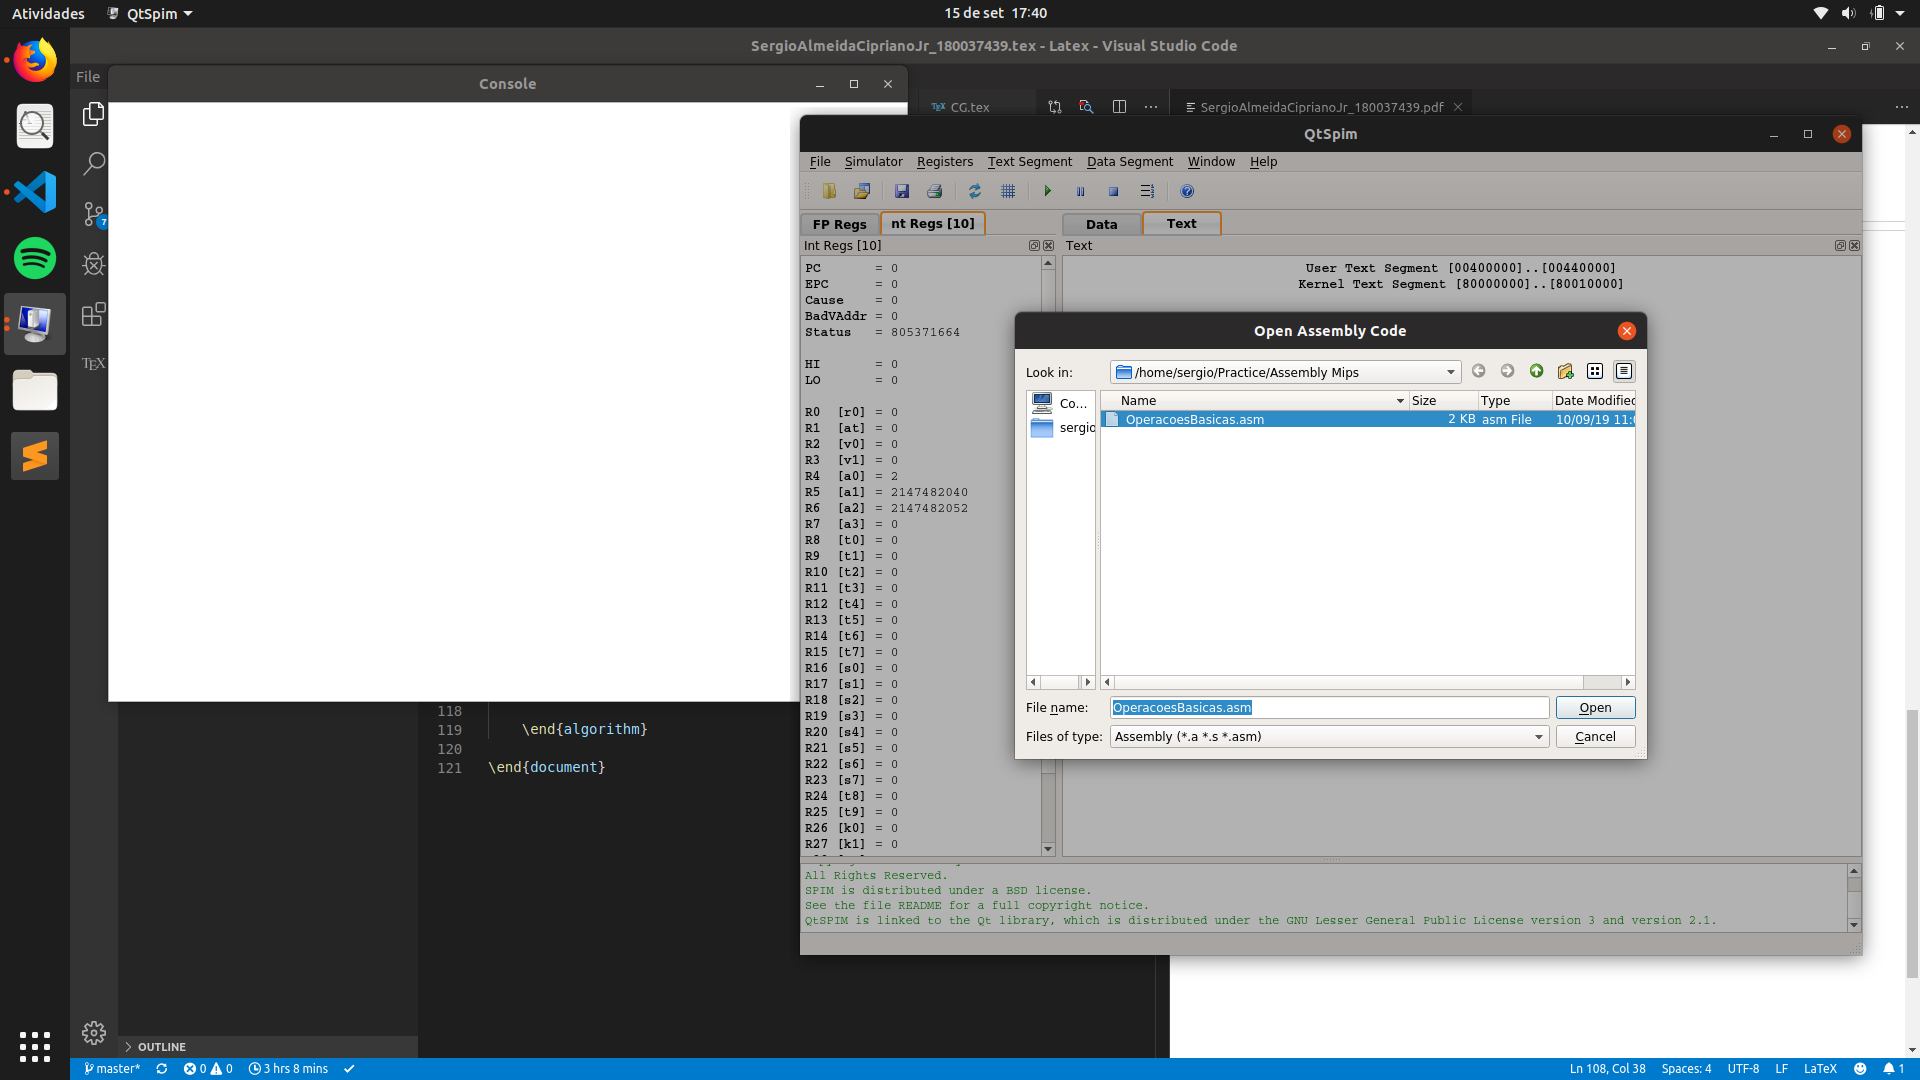
\includegraphics[width=8cm]{Selecionando_arquivo.png}
    \caption{Selecionando arquivo .asm}
    \end{figure}

    \begin{figure}[ht]
    \centering
    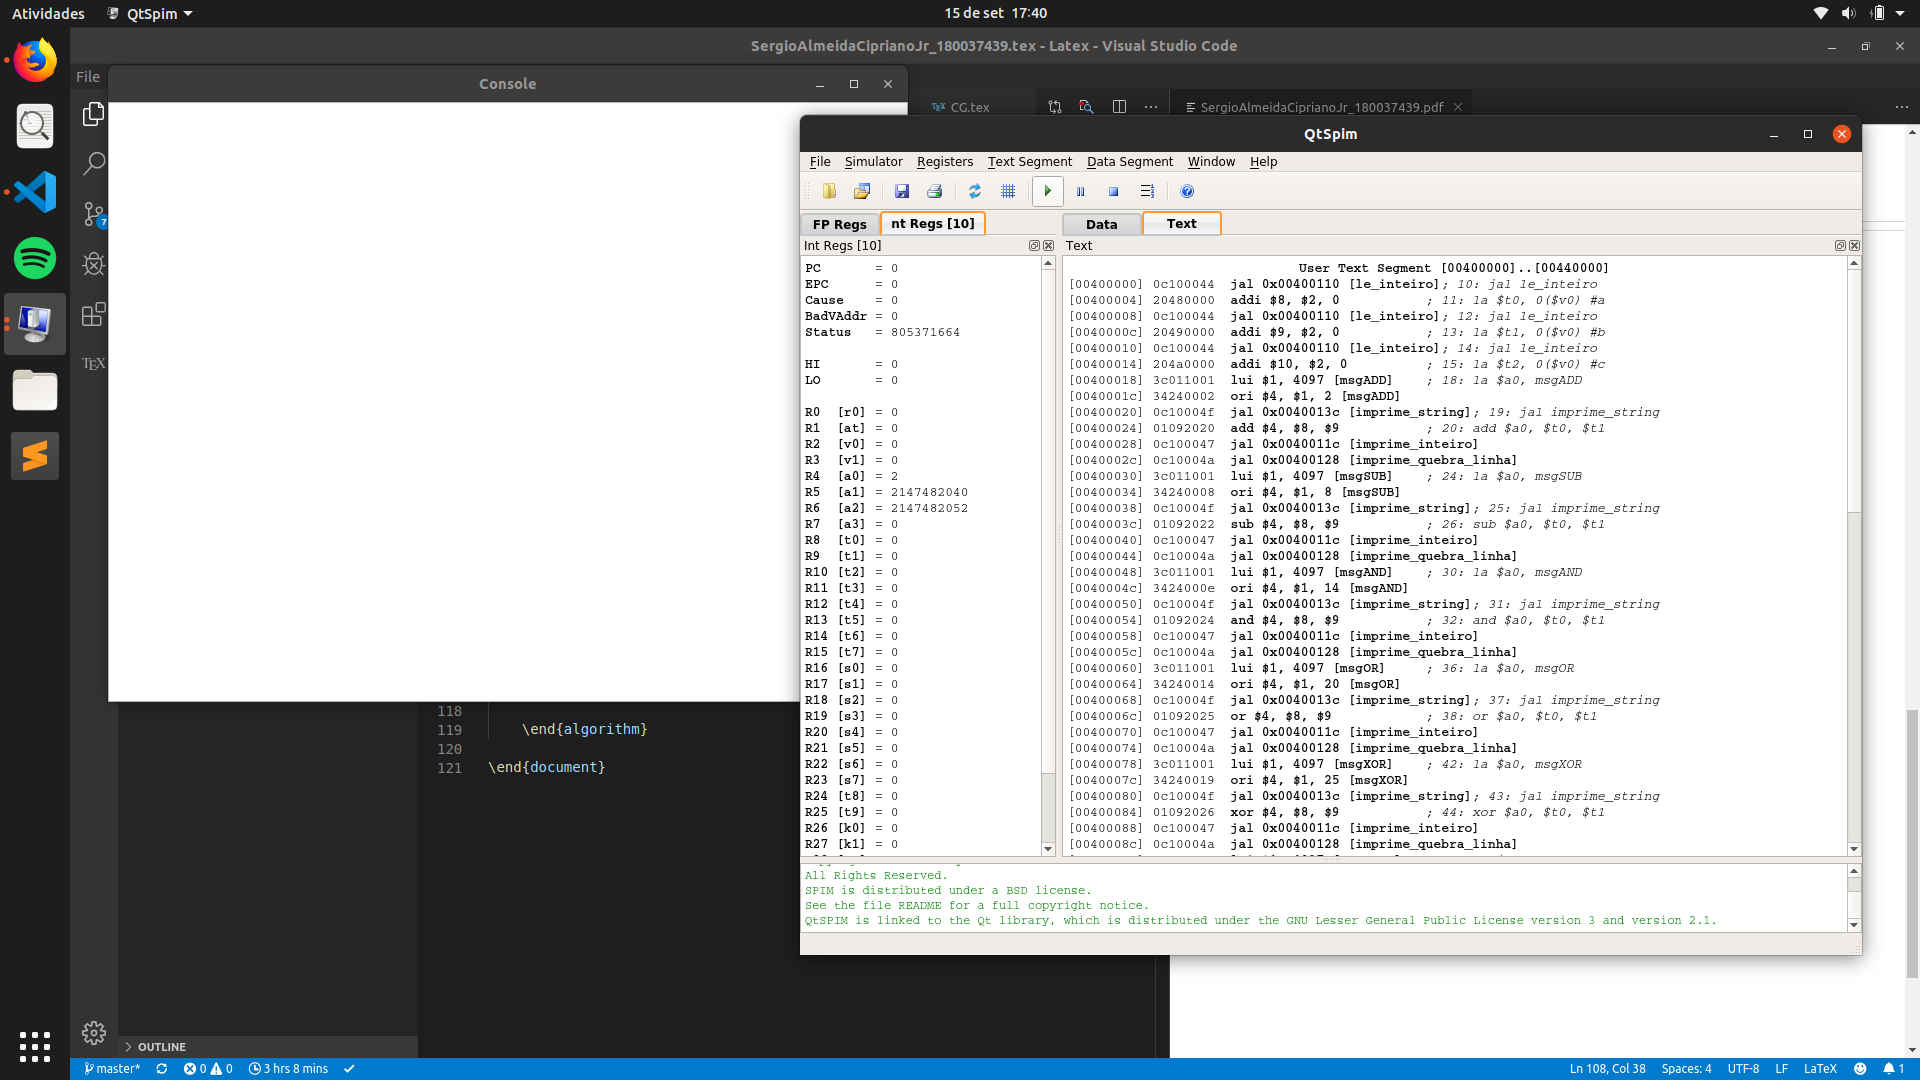
\includegraphics[width=8cm]{Rodando_programa.png}
    \caption{Rodando programa}
    \end{figure}    

    \begin{figure}[ht]
    \centering
    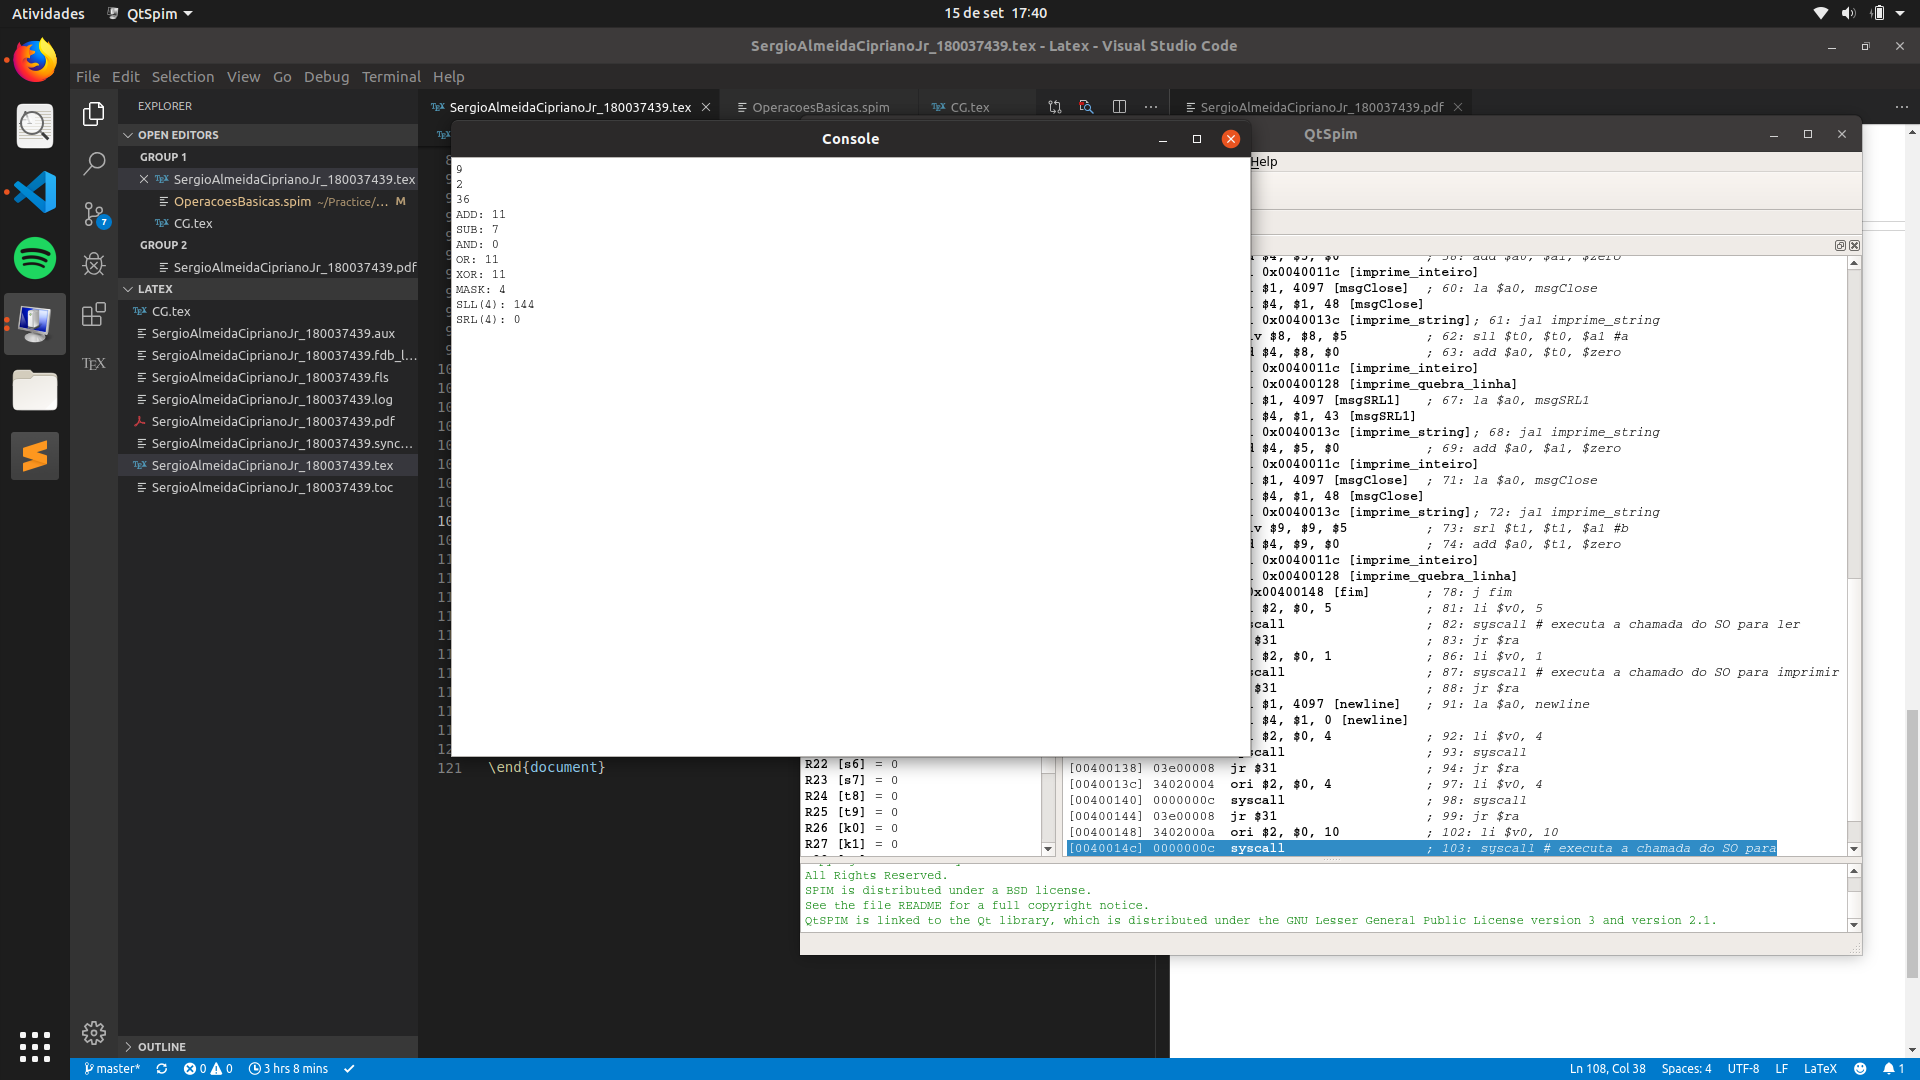
\includegraphics[width=8cm]{Digitando_saida.png}
    \caption{Digitando input}
    \end{figure}

\end{document}